\chapter{测试与阶段结果}

\section{基础环境测试}

环境测试主要验证虚拟环境、OpenCV、smbus2 和项目源码路径是否正常。当前测试中，OpenCV 与 smbus2 均可导入，项目包 \texttt{orangepi\_tracker} 可被 Python 正确识别，单元测试能够通过。测试通过截图如图~\ref{fig:unit-test-ok} 所示。

\begin{figure}[htbp]
  \centering
  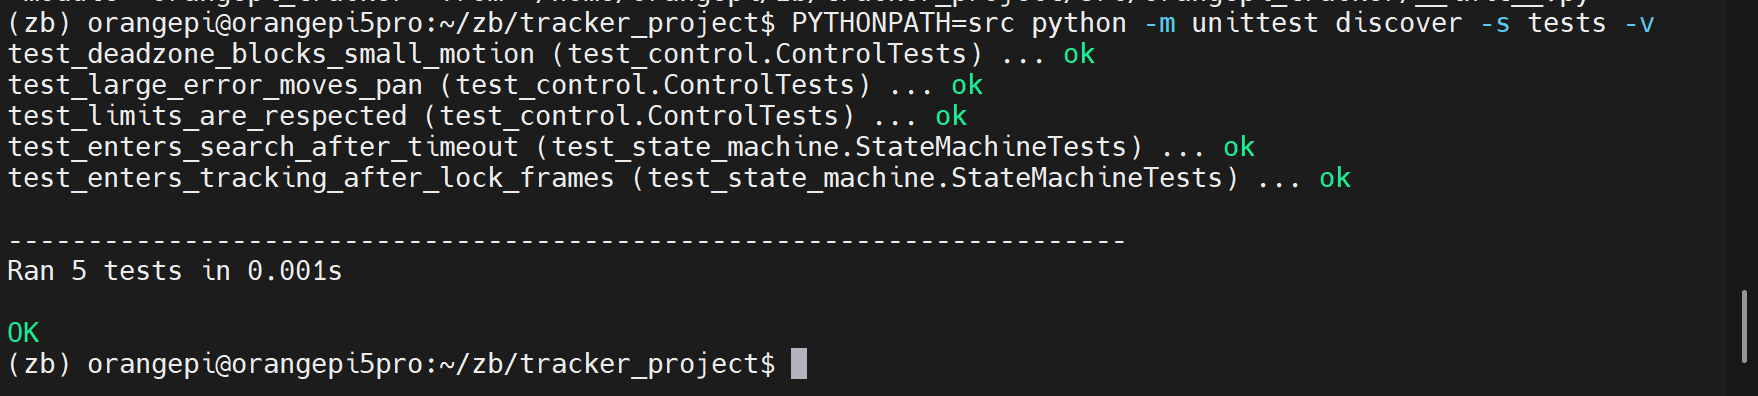
\includegraphics[width=0.86\linewidth]{figures/unit_test_ok.png}
  \caption{基础环境与单元测试结果}
  \label{fig:unit-test-ok}
\end{figure}

\section{摄像头读取测试}

摄像头通过 USB 接入 OrangePi 后，系统可以识别到 \texttt{/dev/video0} 和 \texttt{/dev/video1} 等视频设备。通过 OpenCV 读取测试，\texttt{VideoCapture(0)} 能够打开并读取一帧图像，图像尺寸为 $480 \times 640 \times 3$，说明摄像头硬件和 OpenCV 读取链路正常。

\section{舵机与闭环测试}

舵机测试阶段验证了 PCA9685 通道与云台实际运动方向。当前配置中，俯仰舵机连接 channel 0，水平舵机连接 channel 1。主程序能够控制云台依次运动到设定角度，未出现持续顶住机械结构或失控乱转的问题。

闭环测试阶段，系统能够在红色高对比目标进入画面后识别目标，并根据目标相对画面中心的偏差输出云台控制量。目标短时离开画面时，系统进入短时丢失或搜索状态，而不是立即大幅乱转。

\section{网页监控测试}

网页监控模式已在远程调试场景中跑通。由于 MobaXterm 的 X11 转发在 OpenCV 窗口场景下可能出现显示授权问题，网页监控模式能够有效替代本地图形窗口。通过电脑浏览器访问 OrangePi 的 \texttt{5000} 端口，可以看到带有检测信息和状态信息的实时视频流。

\section{当前问题与不稳定因素}

当前系统已完成主流程打通，但仍存在以下需要继续优化的地方：

\begin{enumerate}
  \item 网页 MJPEG 推流与视觉处理在同一请求循环中执行，当网络波动或浏览器多次连接时可能影响稳定性；
  \item 目标颜色阈值仍依赖固定 HSV 参数，光照变化较大时需要手动调整；
  \item 当前主要跟踪对象为红色高对比标记物，不适合直接泛化到任意目标；
  \item C/C++ 加速模块已经完成初步实现，但仍需在 OrangePi 上构建 wheel 并补充完整性能数据；
  \item 运行日志尚未自动生成曲线图，后续报告中的量化展示仍需补充。
\end{enumerate}

\section{阶段测试结论}

综合当前测试结果，系统已经达到课程大作业的基础演示要求：能够完成摄像头采集、目标检测、双舵机控制和远程监控。下一阶段的重点应从“打通功能”转向“提升稳定性、补全量化数据和完善加分项实验”。

